\documentclass[a4paper]{article}
\usepackage{graphicx}
\usepackage{parskip}
\usepackage{listings}
\usepackage{color}
\usepackage{float}
\usepackage[a4paper]{geometry}

\definecolor{dkgreen}{rgb}{0,0.6,0}
\definecolor{gray}{rgb}{0.5,0.5,0.5}
\definecolor{mauve}{rgb}{0.58,0,0.82}

\lstset{frame=tb,
  language=Python,
  aboveskip=3mm,
  belowskip=3mm,
  showstringspaces=false,
  columns=flexible,
  basicstyle={\small\ttfamily},
  numbers=none,
  numberstyle=\tiny\color{gray},
  keywordstyle=\color{blue},
  commentstyle=\color{dkgreen},
  stringstyle=\color{mauve},
  breaklines=true,
  breakatwhitespace=true,
  tabsize=3
}
\title{Big Data - Credit Scoring}
\title{Assignment Three}
\date{27th March 2017}
\author{Will Peck - wrp3}
\begin{document}
\maketitle
\newpage
\tableofcontents
\newpage
\section{Introduction}
This report discusses the methods used to analyse the credit scoring dataset and attempts to draw some conclusions through the process.

\section{Exploring the Data}
The dataset contains multiple variables used to determine the credit status of indivuals.  The 'CreditStatus' column values are represented in binary representation of true and false where 1 is true, 0 is false.  This attribute is not described in the provided document describing the dataset.  Therefore, it is important to discover this value represents.  Whilst tempting to assume that 0 means rejected and 1 as accepted for a credit application.  It could equally represent 0 for low risk and 1 for high risk.  Further analysis of the attributes that support these values need to be examined.

Some attributes were initially considerred irrelevent to the analysis.  One example of this was 'telephone' which was dropped from the dataframe.  However, for credit risk assessment the customer owning a telephone might be important to lender.  This could be from the perspective of a preference for being able to contact the customer in the future.

By looking at the standard deviation for each of the properties, an understanding of the variability of the data can be established.

\begin{lstlisting}
              Age  ExistingCreditsAtBank  NumberDependents  CreditStatus  \
count  148.000000             148.000000        148.000000    148.000000   
mean     0.352251               0.127280          0.347591      0.716216   
std      0.202610               0.166650          0.472531      0.452364   
min      0.035714               0.000000          0.000000      0.000000   
25%      0.195856               0.000000          0.000000      0.000000   
50%      0.321429               0.000000          0.000000      1.000000   
75%      0.450893               0.333333          1.000000      1.000000   
max      0.982143               0.666667          1.000000      1.000000  
\end{lstlisting}

It could be argued that the variability in the 'Age' column is quite low which could suggest that either; credit applications are applied for by persons residing within a narrow age range or the data capture is not as diverse as it could be.

When using the original dataframe for comparing credit status with age; there is a simularity in the shape of the histograms (figure 1).  However, a credit status of one is awarded to a higher number of people in lower 0.1 to 0.25 range compared to those awarded 0.  These graphs illustrate the previous age range observation and that a conclusion on credit risk could not be evaluated through 'Age' alone.

The attributes that could impact credit worthiness of an individual are contained within the dataset.  The most important qualitative attributes could arguably include:

\begin{itemize}
\item{Housing - This defines the persons residential status and is categorical. The options are 'rent', 'own' or 'for free'.}
\item{Job - Qualitative item that defines current employment status and interesting ly, the type of job is defined: 'unemployed/unskilled - non-resident', 'unskilled - resident', 'skilled employee/official', 'management/self-employed'}
\item{CreditHistory - The credit history of an individual would certainly help to define their credit risk.  This again is categorical data where the options are: 'no credits taken/ all credits paid back duly', 'all credits at this bank paid back duly', 'existing credits paid back duly till now', 'delay in paying off in the past', 'critical account/ other credits existing (not at this bank)'}
\end{itemize}

The numerical (or quantitative) data properties are particularly useful for improving the accurracy of the predictive algorithm where previous loan amount, savings and interest rates can be correlated to the categorical data as outlined above.  Furthermore, the numerical data offers further insight into personal circumstances of the invidual including, for example, the number of dependents. 

The above outlines the attributes that might be the most important for towards assessing credit risk.  Other attributes could serve to assess borderline cases perhaps through a referal process or used to offer more competive interest rates to low risk customers.
   
\begin{figure}[H]
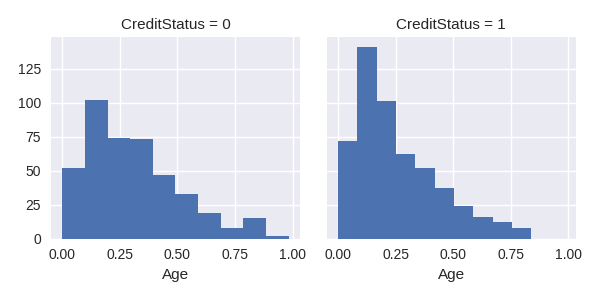
\includegraphics[scale=1]{./barcompareage.png}
\caption{Histogram 'Age' for each 'CreditStatus'.}
\end{figure}

\section{Classification and Evaluation}

The linear regression model initially consisted of all numerical properties within the dataframe.  As a starting point, this gave an opportunity to analyse the performance and build on the accuracy through creating dummy variables to represent categorical data in the model.
\newpage
\begin{lstlisting}
Coefficients:
 [[ 2.20968601  1.557971    0.81231807  0.18801776 -1.54262753 -1.06516558
   0.35303502]]
Intercept: [-0.77293104]
Scores:
 ['0.658', '0.655', '0.714', '0.655', '0.672', '0.619', '0.661', '0.653']
Mean score: 0.66100196434506
Score against training data: 0.6710526315789473
Score against test data: 0.6631578947368421
\end{lstlisting}

\begin{figure}[H]
\begin{center}
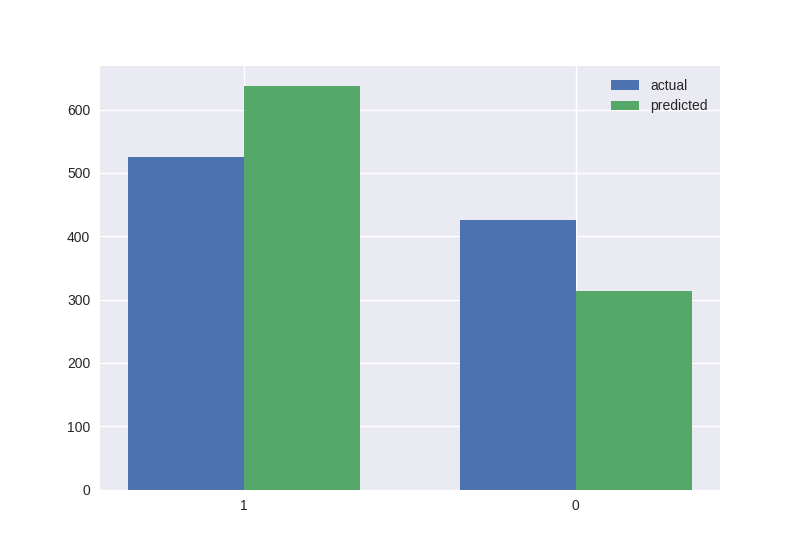
\includegraphics[scale=0.3]{./linnumer.png}
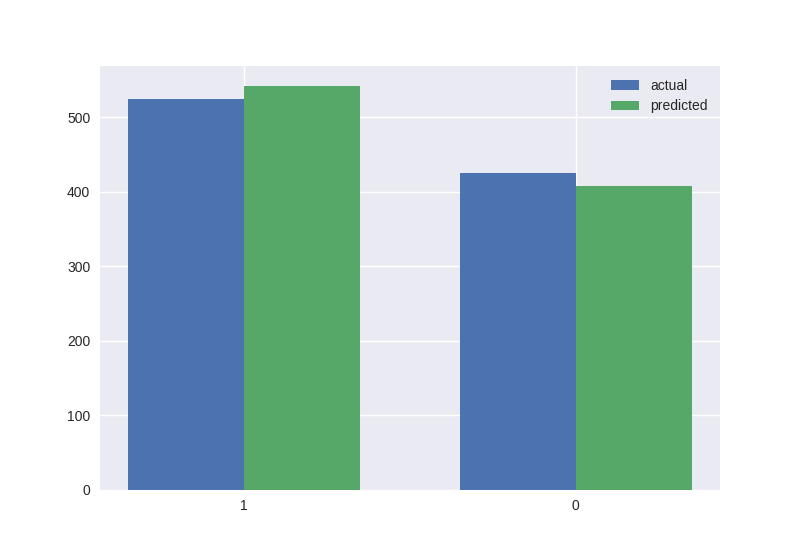
\includegraphics[scale=0.3]{./lincater.png}
\end{center}
\caption{Left: Numeric data only logarithmic regression. Right: Logarithmic regression model including categorical data.}
\end{figure} 

The quantitative data provided a reasonable model but the margin of errow was too high to be useful for credit risk decisions.  The next step was to process the categorical data into a format that could be used in the logistic regression model.  This was achieved with the following code which created columns of boolean values to represent each category definition:
\begin{lstlisting}
...
pd.get_dummies(df, columns=df.select_dtypes(include = [np.object]))
...

Mean score: 0.7632499821962684
Score against training data: 0.7552631578947369
Score against test data: 0.8
\end{lstlisting}

Using the RFE (Recursive Feature Elimination) function, the estimated 12 best features were automatically selected. As an experiment, the RFE result was compared against the manually selected properties highlighted as potentially the most influential as discussed earlier. This suprisingly resulted in a significantly less effective model:

\begin{lstlisting}
RFE = ['Duration', 'CreditAmount', 'InstallmentRatePecnt', 'Age', 'CheckingAcctStat_B', 'CheckingAcctStat_C', 'CreditHistory_D', 'Purpose_D', 'Purpose_H', 'Employment_B', 'OtherDetorsGuarantors_C', 'ForeignWorker_B']

#Results in..

Mean score: 0.7579533720267768
Score against training data: 0.743421052631579
Score against test data: 0.8052631578947368

Manually Selected = ['Duration', 'CreditAmount', 'Age','NumberDependents','ExistingCreditsAtBank', 'Job_A', 'Job_B', 'Job_C', 'Job_D','CreditHistory_A','CreditHistory_B','CreditHistory_C', 'CreditHistory_D',
'CreditHistory_E', 'Housing_A', 'Housing_B','Housing_C', 'Employment_A', 'Employment_B', 'Employment_C', 'Employment_D', 'Employment_E']

#Results in..

Mean score: 0.6768923883112568
Score against training data: 0.6881578947368421
Score against test data: 0.7157894736842105
\end{lstlisting}

\subsection{Logistic Regression Equation}
$
c = 2.59195747 + 1.90917169 + 0.95288228 -1.77938444 -1.73881691 -1.19258039
   1.13152665 + 0.87654111 -1.00329868 -0.88923368 -0.88757393 -2.00359942\\
\\
p = \frac{\exp^{cx}}{1 + \exp^{cx}}
$
\subsection{Receiver Operator Characteristic Curve and Area Under the Curve}
$
AOC = 0.860573111338
$
\begin{figure}[H]
\begin{center}
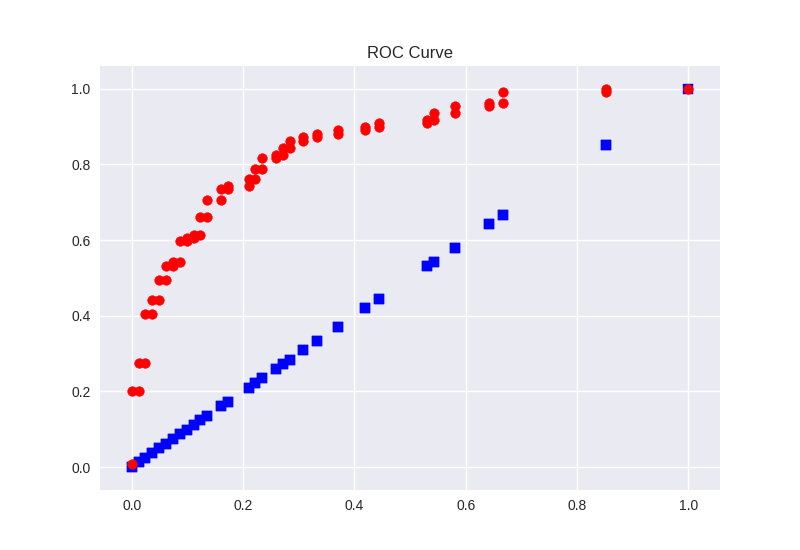
\includegraphics[scale=0.6]{./roc.png}
\end{center}
\caption{The ROC Curve}
\end{figure}

\section{Clustering}

Establishing an optimum number of clusters without forcing a fit to the data was the objective with the implementation of K-means clustering.  Initially, six clusters were generated. Whilst the cluster plots looked tightly bound with no overlap, the differentiation in the data was more difficult to discover.  After trying different amounts, it was concluded that 4 clusters looked the most organic (meant to be natural to what might be expected if additional data was added) whilst still maintaining seperation between clusters and keeping a relatively tight fit.  

\begin{figure}[H]
\begin{center}
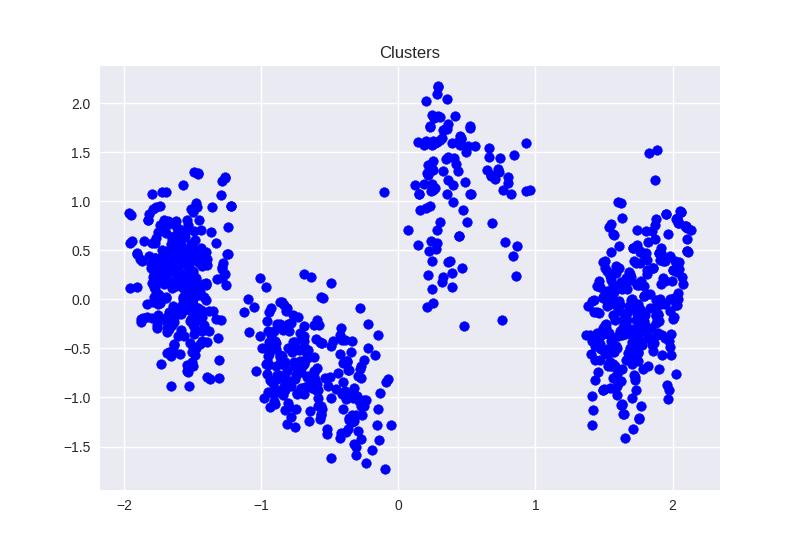
\includegraphics[scale=0.6]{./cluster.png}
\end{center}
\caption{K-Means clustering applied to the dataset.}
\end{figure}

When comparing the clusters; there are identifiable differences between them when comparing properties.  This could allow targeted marketing and perhaps even pre-qualification for credit related products:

\begin{figure}[H]
\begin{center}
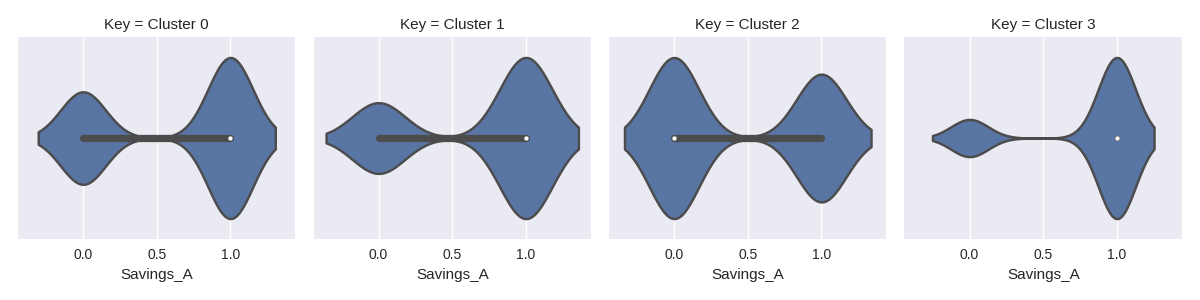
\includegraphics[scale=0.4]{./savings.png}
\end{center}
\caption{Example of defined differences in 'savings' between clusters.}
\end{figure}

\section{Conclusion}
This exercise has provided the opportunity to apply and experiment with different ways to extract meaningful information from large sets of data.  Suprises presented themselves when the certainty of choosing features that were certain to produce the most accurate predictions were proved wrong by RFE.  Furthermore, the K-means algorithm is clearly a fantistic tool for defining groups of entities which should have similar charactistics when used intuitively.  However, it appears that data can be forced to fit by implementing too many clusters which might then not produce realistic results.      
\end{document}
